\documentclass[12pt, a4paper]{report}
\usepackage{amsmath}

\usepackage{graphicx}
\graphicspath{{figures/}}

\title{Machine Learning for Networks}
\author{David Legarre}

\usepackage{booktabs}

\usepackage{units}

\usepackage{multicol}

% Real numbers
\newcommand{\Real}[1]{\mathbb{R}^{#1}}
% Complex numbers
\newcommand{\Complex}[1]{\mathbb{C}^{#1}}
% Integers
\newcommand{\Integer}[1]{\mathbb{Z}^{#1}}

\newtheorem{theorem}{Theorem}

\begin{document}
\maketitle
\chapter{Wifi-networks}
The power transmission of a router is defined with the following formula:
\begin{equation}
   Pt(dBm)=10\log_{10}(Pt[mW])
\end{equation}
Regarding the distance at which the power is lost:
\begin{equation}
   Pl=L1m+10y(f,environment)\log_{10}(d)
\end{equation}
Where $L1m$ is defined as the \textit{Path-loss} at 1 meter (usually $\in\left[ 20,25 \right]$)
\section{Signal to noise ratio}
\begin{figure}[htbp]
   \centering
   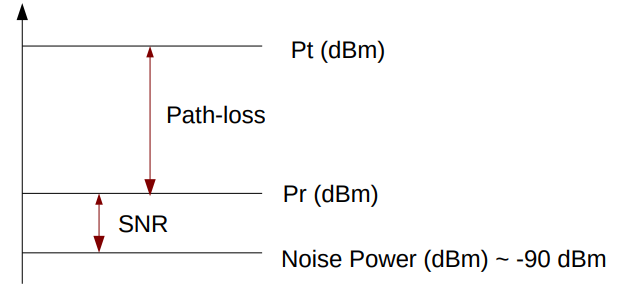
\includegraphics[width=0.8\textwidth]{SNR.png}
   \caption{SNR}
   \label{SNR}
\end{figure}
Defined as:
\begin{equation}
   SNR[dB]=Pr[dBm]-\text{Noise Power}[dBm]
\end{equation}
\end{document}